%! Author = adrienkoumgangtegantchouang
%! Date = 09/06/25


\chapter{Backend Implementation}\label{ch:backend-implementation}


This backend of the \textbf{Smart News Aggregator} is built using \textbf{Flask} (Python) with \textbf{Flask-RESTX} for API development.


\section{System Architecture}\label{sec:system-architecture}


\subsection{Key Components}\label{subsec:backend-key-components}

\begin{tabular}{lll}
  \toprule
  Component & Technology & Purpose \\
  \midrule
  API Server & Flask\cite{flask, flaskrestx} + Gunicor & HTTP request handling \\
  Auth & JWT(RS256)\cite{jwt}  & User authentication \\
  Caching & Redis & Session/store hot data \\
  Asybc Tasks & Flask Cron & Background jobs (API fetching) \\
  Docs & Swagger UI\cite{swagger} & Interactive API documentation \\
  \bottomrule
\end{tabular}


\section{API Endpoints}\label{sec:api-endpoints}


\subsection{Authentication}\label{subsec:authentication}

\begin{tabularx}{\textwidth}{lcX}
  \toprule
  Endpoint & Method & Description \\
  \midrule
  $/auth/register$ & POST & User registration \\
  $/auth/login$ & POST  & JWT token generation \\
  $/auth/login-alt$ & POST & JWT token generation without password validation \\
  $/auth/change\_password$ & POST & Update user password \\
  $/auth/me$ & GET & Get current user information like email, name, status, role \\
  \bottomrule
\end{tabularx}

\begin{figure}[!h]
    \centering
    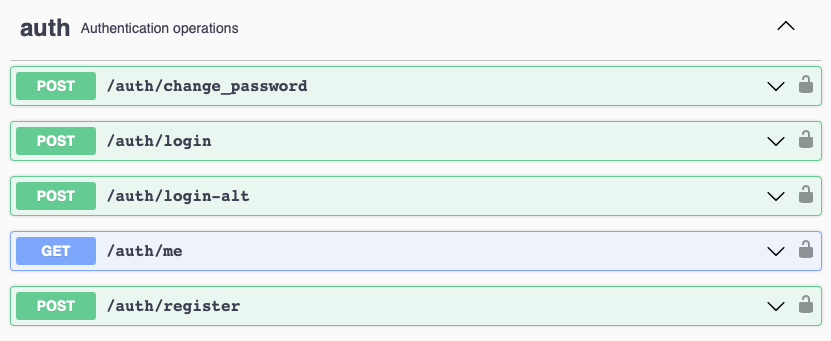
\includegraphics[width=1\textwidth]{chapters/chapter_06/authentication-operations}
    \caption{API Endpoint: Authentication endpoint}
    \label{fig:api-authentication-endpoint}
\end{figure}


\subsection{User Management}\label{subsec:user-management}


\begin{tabularx}{\textwidth}{lcX}
  \toprule
  Endpoint & Method & Description \\
  \midrule
  $/user/article/preference$ & POST & Add article preference tags for current user \\
  $/user/article/preference$ & GET & Get article preference tags for current user \\
  $/user/me$ & POST & Update current user information \\
  $/user/me$ & GET & Get current user information \\
  \bottomrule
\end{tabularx}

\begin{figure}[!h]
    \centering
    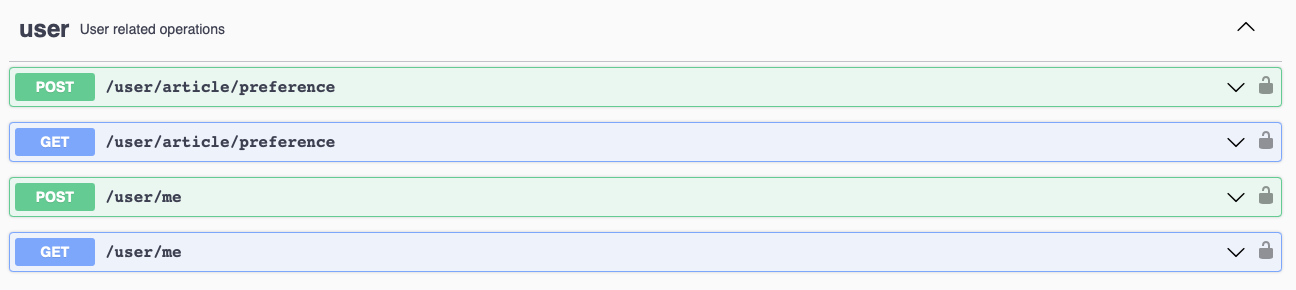
\includegraphics[width=1\textwidth]{chapters/chapter_06/user-operations}
    \caption{API Endpoint: User endpoint}
    \label{fig:api-user-endpoint}
\end{figure}


\subsection{Article Management}\label{subsec:article-management}

\begin{tabularx}{\textwidth}{XcX}
  \toprule
  Endpoint & Method & Description \\
  \midrule
  $/article/comment/me$ & GET & List of comment make by current user \\
  $/article/history$ & GET & List of read articles \\
  $/article/latest$ & GET & List of all articles order by recent published \\
  $/article/search$ & GET & List of article where title or description content query \\
  $/article/tags$ & POST & - \\
  $/article/tags$ & GET & - \\
  $/article/\{article\_id\}$ & GET & Get all article data \\
  $/article/\{article\_id\}/comment$ & POST & Add comment on article \\
  $/article/\{article\_id\}/comment$ & GET & List of comment for this specific article \\
  $/article/\{article\_id\}/comment/$ $\{comment\_id\}$ & GET & Get all comment data \\
  $/article/\{article\_id\}/comment/$ $\{comment\_id\}$ & DELETE & Delete specific comment \\
  $/article/\{article\_id\}/comment/$ $\{comment\_id\}/interaction$ & POST & add interaction in this comment \\
  $/article/\{article\_id\}/comment/$ $\{comment\_id\}/interaction$ & GET & Get interaction information in this comment \\
  $/article/\{article\_id\}/interaction$ & POST & Add interaction in this article \\
  $/article/\{article\_id\}/interaction$ & GET & Get article interaction information \\
  $/article/\{article\_id\}/summary$ & GET & Get summable details of this article \\
  \bottomrule
\end{tabularx}


\begin{figure}[!h]
    \centering
    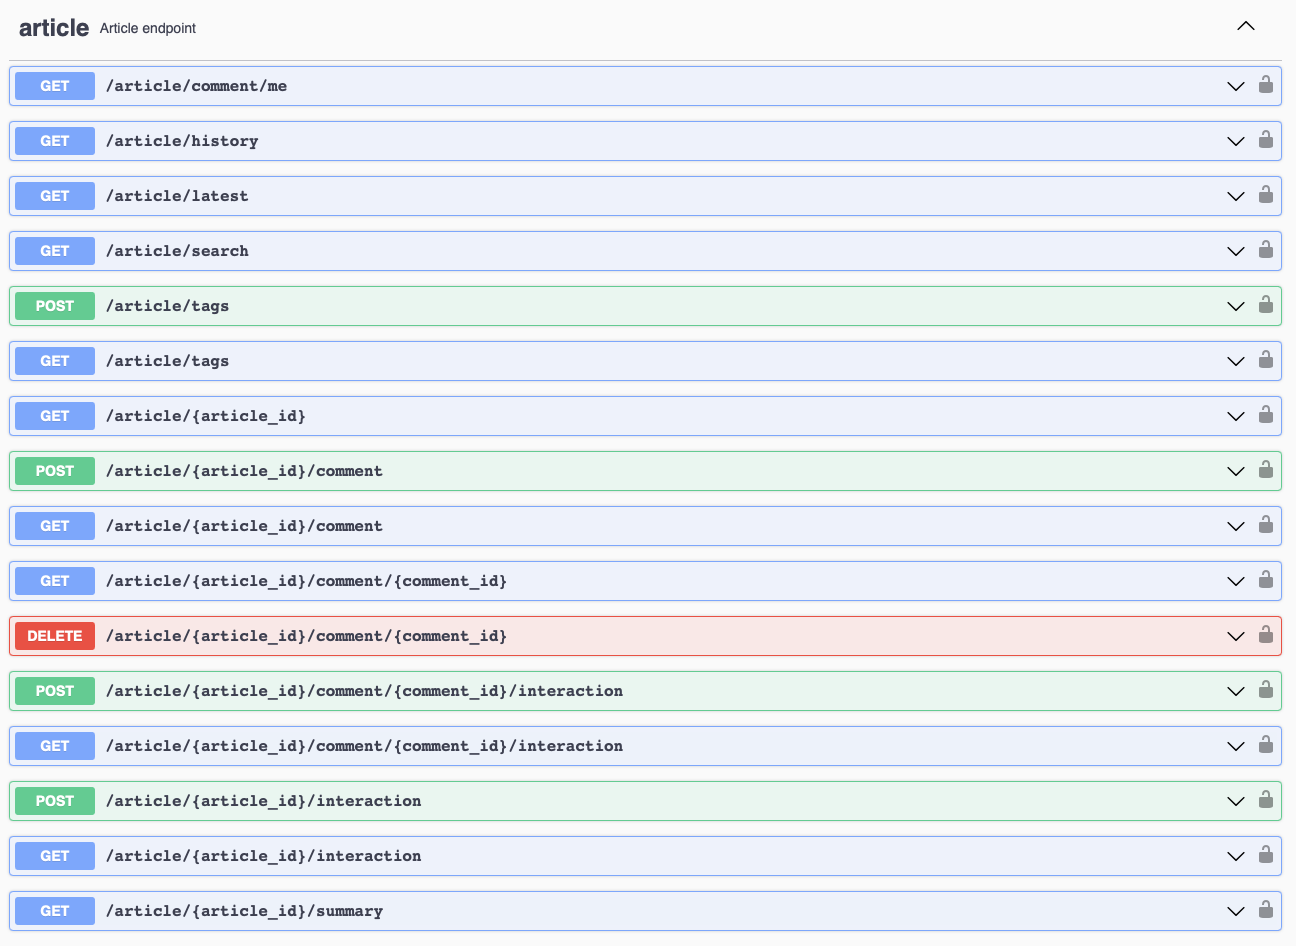
\includegraphics[width=1\textwidth]{chapters/chapter_06/articles-operations}
    \caption{API Endpoint: Articles endpoint}
    \label{fig:api-articles-endpoint}
\end{figure}


\subsection{Administration Management}\label{subsec:admin-management}

\begin{tabularx}{\textwidth}{XcX}
  \toprule
  Endpoint & Method & Description \\
  \midrule
  $/admin/article/\{article\_id\}$ & DELETE & Delete Article \\
  $/admin/articles$ & GET & List of all articles \\
  $/admin/dashboard/errors$ & GET & List of log of errors occur in server during execution \\
  $/admin/dashboard/errors/$ $\{server\_error\_log\_id\}$ & DELETE & delete server error log \\
  $/admin/users$ & GET & List of all users \\
  $/admin/user/\{user\_id\}$ & GET & Get all user data \\
  $/admin/user/\{user\_id\}$ & PUT & Add user \\
  $/admin/user/\{user\_id\}$ & POST & Update user \\
  $/admin/user/\{user\_id\}$ & DELETE & Delete User \\
  $/admin/$ & GET & - \\
  \bottomrule
\end{tabularx}

\begin{figure}[!h]
    \centering
    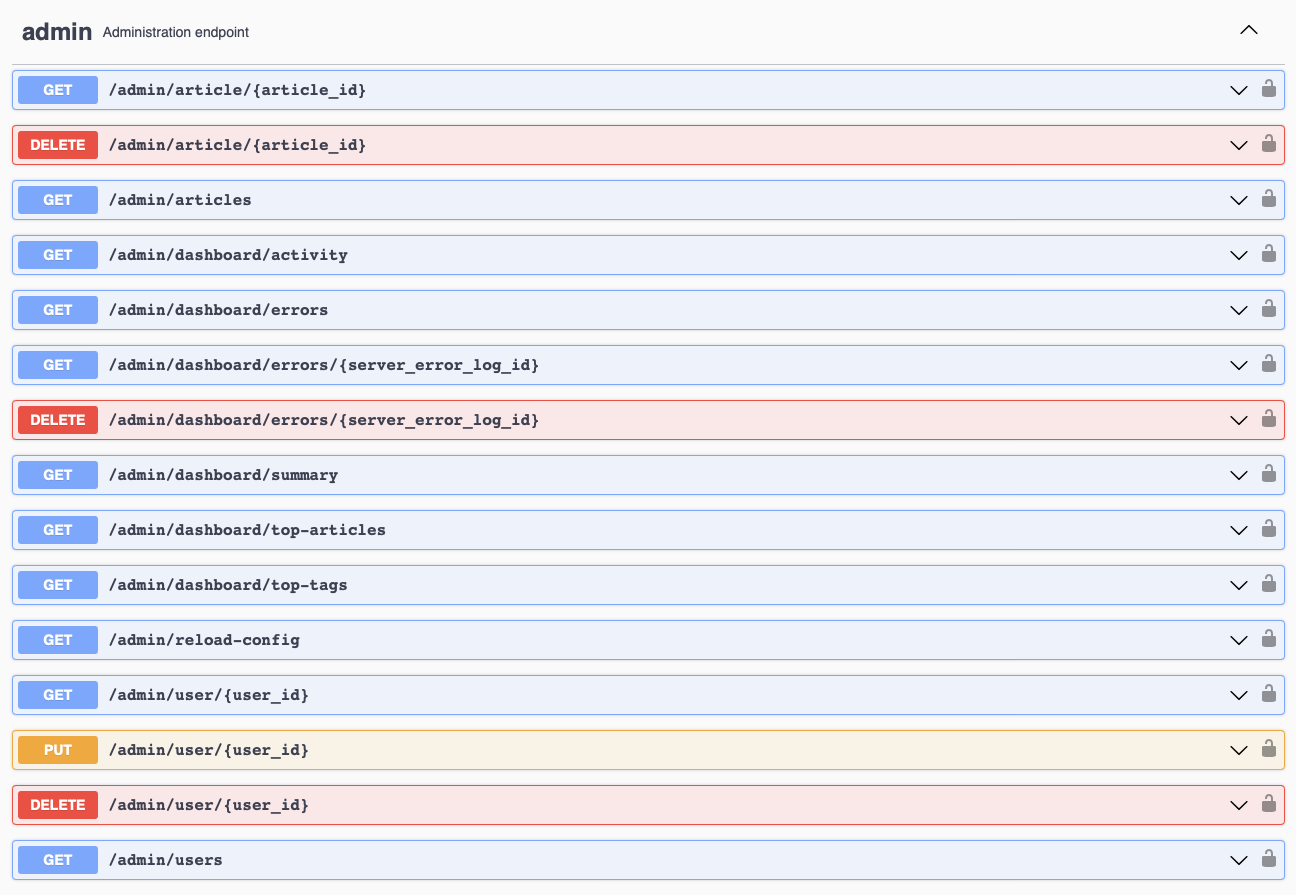
\includegraphics[width=1\textwidth]{chapters/chapter_06/admin-operations}
    \caption{API Endpoint: Admin endpoint}
    \label{fig:api-admin-endpoint}
\end{figure}


\section{Security Implementation}\label{sec:security-implementation}

\subsection{JWT Authentication}\label{subsec:jwt-authentication}

\textbf{Algorithm RS256 (asymmetric)} for token and \textbf{validation middleware}:

\begin{lstlisting}[style=pythonstyle,label={lst:decoration-token-required},caption={Decoration 'Token Required'}]
def token_required(f):
    @wraps(f)
    def decorated(*args, **kwargs):
        token = None

        # Extract token from Authorization header
        auth_header = request.headers.get('Authorization', '')
        if auth_header.startswith("Bearer "):
            token = auth_header.split(" ")[1]

        if not token:
            return {'error': 'Token is missing!'}, 401

        try:
            user = TokenManager.decode_token(token=token)

            if 'admin' in request.url and user.role != 'admin':
                raise UnauthorizedException('You are not authorized to perform this operation')

            g.user = user
        except TokenException as e:
            return {'error': str(e)}, 401

        return f(*args, **kwargs)

    return decorated
\end{lstlisting}

\subsection{Input Validation}\label{subsec:input-validation}

All input data is validated via flask-rest's marshal service, which ensures the integrity of input data.

\begin{lstlisting}[style=pythonstyle,label={lst:input-validation-with-marshal},caption={Input validation with marshal}]
@ns_article.route('/<string:article_id>/interaction')
@ns_article.param('article_id', 'The article ID')
class ArticleInteractionResource(Resource):
    @token_required
    @ns_article.expect(ArticleInteractionType.to_model(name_space=ns_article))
    @ns_article.marshal_with(Model.get_message_response_model(name_space=ns_article))
    def post(self, article_id):
        user_token: UserToken = g.user

        data = request.get_json()
        interaction = ArticleInteractionType(**data)
        result = UserArticleInteractionModel.update_interaction(user_token, interaction=interaction, article_id=article_id)

        if result:
            return {"success": True, "message": "Interaction updated"}
        return {"success": False, "message": "Interaction could not be updated"}
\end{lstlisting}


\section{Performance Optimizations}\label{sec:performance-optimizations}

\subsection{Caching Strategies}\label{subsec:caching-strategies}

\begin{tabularx}{\textwidth}{lXl}
  \toprule
  Cache Key & Data & TTL \\
  \midrule
  $user:\<user\_id\>$ & Full user json & - \\
  $article:\<article\_id\>$ & - & - \\
  $article:last:count$ & all last articles count & - \\
  $article:last:\<user\_id\>:count$ & all last articles count with user preferences & - \\
  $article:last:\<page\>:\<limit\>$ & full list last articles json by page and limit & - \\
  $article:all:count$ & all articles count & - \\
  $article:all:\<page\>:\<limit\>$ & full list articles json by page and limit & - \\
  $comment:all:\<filter\>:\<page\>:\<limit\>$ & full list comment by article, page and limit  & - \\
  \bottomrule
\end{tabularx}

\subsection{Async Task Processing}\label{subsec:async-task-processing}

When a user accesses a list of items via services such as latest, history, each item in the list is cached.

\begin{lstlisting}[style=pythonstyle,label={lst:async-cache-article},caption={Async Cache Article}]
class ArticleModel(ArticleSummaryModel):
    @classmethod
    def _cache_articles(cls, user_token: UserToken, articles: list):
        for article in articles:
            _ = cls.get(user_token, str(article.article_id))

    @classmethod
    def cache_articles(cls, user_token: UserToken, articles: list):
        thread = Thread(target=cls._cache_articles, args=(user_token, articles,))
        thread.daemon = True
        thread.start()
\end{lstlisting}


\section{API Documentation}\label{sec:api-documentation}

My api's documentation is auto-generated using flask-restx namesapces and swagger accessible via swagger ui via endpoint /api/docs.

\begin{lstlisting}[style=pythonstyle,label={lst:api-documentation-article-summary},caption={Api Docuentation Article Summary}]
class ArticleSummaryModel(MongoDBBaseModel):
    @staticmethod
    def to_model(name_space: Namespace):
        return name_space.model('ArticleSummaryModel', {
            'article_id': fields.String(required=False),
            'extern_id': fields.String(required=False),
            'extern_api': fields.String(required=True),
            'title': fields.String(required=True),
            'description': fields.String(required=True),
            'author': fields.Nested(ArticleSourceModel.to_model(name_space)),
            'source': fields.Nested(ArticleSourceModel.to_model(name_space)),
            'image_url': fields.String(required=True),
            'published_at': fields.String(required=True),
            'tags': fields.List(fields.String, description="List of tags"),
            'current_user_interaction': fields.Nested(ArticleInteractionStatus.to_model(name_space)),
            'total_user_interaction': fields.Nested(ArticleInteractionStats.to_model(name_space)),
        })

    @staticmethod
    def to_model_list(name_space: Namespace):
        return name_space.model('ArticleSummaryModelList', {
            'articles': fields.List(fields.Nested(ArticleSummaryModel.to_model(name_space)),),
            'total': fields.Integer,
            'page': fields.Integer,
            'limit': fields.Integer,
            'pageCount': fields.Integer,
        })
\end{lstlisting}






